\batchmode
\documentclass[twoside]{book}

% Packages required by doxygen
\usepackage{fixltx2e}
\usepackage{calc}
\usepackage{doxygen}
\usepackage[export]{adjustbox} % also loads graphicx
\usepackage{graphicx}
\usepackage[utf8]{inputenc}
\usepackage{makeidx}
\usepackage{multicol}
\usepackage{multirow}
\PassOptionsToPackage{warn}{textcomp}
\usepackage{textcomp}
\usepackage[nointegrals]{wasysym}
\usepackage[table]{xcolor}

% Font selection
\usepackage[T1]{fontenc}
\usepackage[scaled=.90]{helvet}
\usepackage{courier}
\usepackage{amssymb}
\usepackage{sectsty}
\renewcommand{\familydefault}{\sfdefault}
\allsectionsfont{%
  \fontseries{bc}\selectfont%
  \color{darkgray}%
}
\renewcommand{\DoxyLabelFont}{%
  \fontseries{bc}\selectfont%
  \color{darkgray}%
}
\newcommand{\+}{\discretionary{\mbox{\scriptsize$\hookleftarrow$}}{}{}}

% Page & text layout
\usepackage{geometry}
\geometry{%
  a4paper,%
  top=2.5cm,%
  bottom=2.5cm,%
  left=2.5cm,%
  right=2.5cm%
}
\tolerance=750
\hfuzz=15pt
\hbadness=750
\setlength{\emergencystretch}{15pt}
\setlength{\parindent}{0cm}
\setlength{\parskip}{3ex plus 2ex minus 2ex}
\makeatletter
\renewcommand{\paragraph}{%
  \@startsection{paragraph}{4}{0ex}{-1.0ex}{1.0ex}{%
    \normalfont\normalsize\bfseries\SS@parafont%
  }%
}
\renewcommand{\subparagraph}{%
  \@startsection{subparagraph}{5}{0ex}{-1.0ex}{1.0ex}{%
    \normalfont\normalsize\bfseries\SS@subparafont%
  }%
}
\makeatother

% Headers & footers
\usepackage{fancyhdr}
\pagestyle{fancyplain}
\fancyhead[LE]{\fancyplain{}{\bfseries\thepage}}
\fancyhead[CE]{\fancyplain{}{}}
\fancyhead[RE]{\fancyplain{}{\bfseries\leftmark}}
\fancyhead[LO]{\fancyplain{}{\bfseries\rightmark}}
\fancyhead[CO]{\fancyplain{}{}}
\fancyhead[RO]{\fancyplain{}{\bfseries\thepage}}
\fancyfoot[LE]{\fancyplain{}{}}
\fancyfoot[CE]{\fancyplain{}{}}
\fancyfoot[RE]{\fancyplain{}{\bfseries\scriptsize Generated by Doxygen }}
\fancyfoot[LO]{\fancyplain{}{\bfseries\scriptsize Generated by Doxygen }}
\fancyfoot[CO]{\fancyplain{}{}}
\fancyfoot[RO]{\fancyplain{}{}}
\renewcommand{\footrulewidth}{0.4pt}
\renewcommand{\chaptermark}[1]{%
  \markboth{#1}{}%
}
\renewcommand{\sectionmark}[1]{%
  \markright{\thesection\ #1}%
}

% Indices & bibliography
\usepackage{natbib}
\usepackage[titles]{tocloft}
\setcounter{tocdepth}{3}
\setcounter{secnumdepth}{5}
\makeindex

% Hyperlinks (required, but should be loaded last)
\usepackage{ifpdf}
\ifpdf
  \usepackage[pdftex,pagebackref=true]{hyperref}
\else
  \usepackage[ps2pdf,pagebackref=true]{hyperref}
\fi
\hypersetup{%
  colorlinks=true,%
  linkcolor=blue,%
  citecolor=blue,%
  unicode%
}

% Custom commands
\newcommand{\clearemptydoublepage}{%
  \newpage{\pagestyle{empty}\cleardoublepage}%
}

\usepackage{caption}
\captionsetup{labelsep=space,justification=centering,font={bf},singlelinecheck=off,skip=4pt,position=top}

%===== C O N T E N T S =====

\begin{document}

% Titlepage & ToC
\hypersetup{pageanchor=false,
             bookmarksnumbered=true,
             pdfencoding=unicode
            }
\pagenumbering{alph}
\pagenumbering{arabic}
\hypersetup{pageanchor=true}

%--- Begin generated contents ---
\chapter{Demo problem\+: Free, small-\/amplitude axisymmetric oscillation of 2D circular disk}
\label{index}\hypertarget{index}{}\hypertarget{index_q}{}\section{A few quick questions...}\label{index_q}
Since {\ttfamily oomph-\/lib} is developed as open-\/source software, any evidence that the code is being downloaded and used is very helpful for us as it helps to justify our continued work on this project.

We would therefore be extremely grateful if you could provide the information requested in the form below. Pressing the \char`\"{}submit\char`\"{} button will get you to the actual download page.

{\bfseries Note\+:} 
\begin{DoxyItemize}
\item All information will be treated as confidential. 
\item If you provide your email address and check the appropriate box we will add you to our mailing list to inform you of upgrades and bug fixes to the code. Rest assured that the mailing list is {\bfseries very low volume} -- we have better things to do than to bombard you with email. 
\item If you still feel reluctant to provide any of the information requested, feel free to enter some dummy input. The form will check that {\bfseries some} information has been entered but entering your name as \char`\"{}\+Joe Cool\char`\"{} is perfectly acceptable -- this is to discourage people from not providing the information simply because they are too lazy to type... 
\end{DoxyItemize}



 







 

 \hypertarget{index_pdf}{}\section{P\+D\+F file}\label{index_pdf}
A \href{../latex/refman.pdf}{\tt pdf version} of this document is available. \end{document}

\chapter{Namespace Index}
\section{Namespace List}
Here is a list of all namespaces with brief descriptions\+:\begin{DoxyCompactList}
\item\contentsline{section}{\hyperlink{namespaceGlobal__Physical__Variables}{Global\+\_\+\+Physical\+\_\+\+Variables} \\*Global variables that represent physical properties }{\pageref{namespaceGlobal__Physical__Variables}}{}
\item\contentsline{section}{\hyperlink{namespaceoomph}{oomph} }{\pageref{namespaceoomph}}{}
\item\contentsline{section}{\hyperlink{namespacePhysical__Variables}{Physical\+\_\+\+Variables} \\*Namespace for the solution of 2D linear shell equation }{\pageref{namespacePhysical__Variables}}{}
\end{DoxyCompactList}

\chapter{Hierarchical Index}
\section{Class Hierarchy}
This inheritance list is sorted roughly, but not completely, alphabetically\+:\begin{DoxyCompactList}
\item Problem\begin{DoxyCompactList}
\item \contentsline{section}{Unstructured\+Solid\+Problem$<$ E\+L\+E\+M\+E\+NT $>$}{\pageref{classUnstructuredSolidProblem}}{}
\end{DoxyCompactList}
\end{DoxyCompactList}

\chapter{Class Index}
\section{Class List}
Here are the classes, structs, unions and interfaces with brief descriptions\+:\begin{DoxyCompactList}
\item\contentsline{section}{\hyperlink{classPMLProblem}{P\+M\+L\+Problem$<$ E\+L\+E\+M\+E\+N\+T $>$} }{\pageref{classPMLProblem}}{}
\item\contentsline{section}{\hyperlink{classGlobalParameters_1_1TestPMLMapping}{Global\+Parameters\+::\+Test\+P\+M\+L\+Mapping} }{\pageref{classGlobalParameters_1_1TestPMLMapping}}{}
\end{DoxyCompactList}

\chapter{File Index}
\section{File List}
Here is a list of all files with brief descriptions\+:\begin{DoxyCompactList}
\item\contentsline{section}{\hyperlink{jeffery__orbit_8cc}{jeffery\+\_\+orbit.\+cc} }{\pageref{jeffery__orbit_8cc}}{}
\item\contentsline{section}{\hyperlink{jeffery__orbit_8txt__doxygenified_8h}{jeffery\+\_\+orbit.\+txt\+\_\+doxygenified.\+h} }{\pageref{jeffery__orbit_8txt__doxygenified_8h}}{}
\item\contentsline{section}{\hyperlink{my__taylor__hood__elements_8h}{my\+\_\+taylor\+\_\+hood\+\_\+elements.\+h} }{\pageref{my__taylor__hood__elements_8h}}{}
\end{DoxyCompactList}

\chapter{Namespace Documentation}
\hypertarget{namespaceGlobal__Physical__Variables}{}\section{Global\+\_\+\+Physical\+\_\+\+Variables Namespace Reference}
\label{namespaceGlobal__Physical__Variables}\index{Global\+\_\+\+Physical\+\_\+\+Variables@{Global\+\_\+\+Physical\+\_\+\+Variables}}


Namespace for physical parameters.  


\subsection*{Functions}
\begin{DoxyCompactItemize}
\item 
Vector$<$ double $>$ \hyperlink{namespaceGlobal__Physical__Variables_afae321364975eb56688ad13abc8ed6b7}{Gravity} (2)
\begin{DoxyCompactList}\small\item\em Gravity vector. \end{DoxyCompactList}\item 
void \hyperlink{namespaceGlobal__Physical__Variables_a87da705b8a46bed337cf5dbdd788b87b}{body\+\_\+force} (const double \&time, const Vector$<$ double $>$ \&x, Vector$<$ double $>$ \&result)
\begin{DoxyCompactList}\small\item\em Functional body force. \end{DoxyCompactList}\item 
void \hyperlink{namespaceGlobal__Physical__Variables_a9780d615ae07c4e00a436ab2973b54e6}{zero\+\_\+body\+\_\+force} (const double \&time, const Vector$<$ double $>$ \&x, Vector$<$ double $>$ \&result)
\begin{DoxyCompactList}\small\item\em Zero functional body force. \end{DoxyCompactList}\end{DoxyCompactItemize}
\subsection*{Variables}
\begin{DoxyCompactItemize}
\item 
double \hyperlink{namespaceGlobal__Physical__Variables_ab814e627d2eb5bc50318879d19ab16b9}{Re} =100
\begin{DoxyCompactList}\small\item\em Reynolds number. \end{DoxyCompactList}\item 
double \hyperlink{namespaceGlobal__Physical__Variables_ab1a845a672b4d74b304639a976dc65c6}{Re\+\_\+inv\+Fr} =100
\begin{DoxyCompactList}\small\item\em Reynolds/\+Froude number. \end{DoxyCompactList}\end{DoxyCompactItemize}


\subsection{Detailed Description}
Namespace for physical parameters. 

\subsection{Function Documentation}
\mbox{\Hypertarget{namespaceGlobal__Physical__Variables_a87da705b8a46bed337cf5dbdd788b87b}\label{namespaceGlobal__Physical__Variables_a87da705b8a46bed337cf5dbdd788b87b}} 
\index{Global\+\_\+\+Physical\+\_\+\+Variables@{Global\+\_\+\+Physical\+\_\+\+Variables}!body\+\_\+force@{body\+\_\+force}}
\index{body\+\_\+force@{body\+\_\+force}!Global\+\_\+\+Physical\+\_\+\+Variables@{Global\+\_\+\+Physical\+\_\+\+Variables}}
\subsubsection{\texorpdfstring{body\+\_\+force()}{body\_force()}}
{\footnotesize\ttfamily void Global\+\_\+\+Physical\+\_\+\+Variables\+::body\+\_\+force (\begin{DoxyParamCaption}\item[{const double \&}]{time,  }\item[{const Vector$<$ double $>$ \&}]{x,  }\item[{Vector$<$ double $>$ \&}]{result }\end{DoxyParamCaption})}



Functional body force. 



Definition at line 62 of file circular\+\_\+driven\+\_\+cavity.\+cc.



References Re\+\_\+inv\+Fr.



Referenced by main().

\mbox{\Hypertarget{namespaceGlobal__Physical__Variables_afae321364975eb56688ad13abc8ed6b7}\label{namespaceGlobal__Physical__Variables_afae321364975eb56688ad13abc8ed6b7}} 
\index{Global\+\_\+\+Physical\+\_\+\+Variables@{Global\+\_\+\+Physical\+\_\+\+Variables}!Gravity@{Gravity}}
\index{Gravity@{Gravity}!Global\+\_\+\+Physical\+\_\+\+Variables@{Global\+\_\+\+Physical\+\_\+\+Variables}}
\subsubsection{\texorpdfstring{Gravity()}{Gravity()}}
{\footnotesize\ttfamily Vector$<$double$>$ Global\+\_\+\+Physical\+\_\+\+Variables\+::\+Gravity (\begin{DoxyParamCaption}\item[{2}]{ }\end{DoxyParamCaption})}



Gravity vector. 



Referenced by main(), and Quarter\+Circle\+Driven\+Cavity\+Problem$<$ E\+L\+E\+M\+E\+N\+T $>$\+::\+Quarter\+Circle\+Driven\+Cavity\+Problem().

\mbox{\Hypertarget{namespaceGlobal__Physical__Variables_a9780d615ae07c4e00a436ab2973b54e6}\label{namespaceGlobal__Physical__Variables_a9780d615ae07c4e00a436ab2973b54e6}} 
\index{Global\+\_\+\+Physical\+\_\+\+Variables@{Global\+\_\+\+Physical\+\_\+\+Variables}!zero\+\_\+body\+\_\+force@{zero\+\_\+body\+\_\+force}}
\index{zero\+\_\+body\+\_\+force@{zero\+\_\+body\+\_\+force}!Global\+\_\+\+Physical\+\_\+\+Variables@{Global\+\_\+\+Physical\+\_\+\+Variables}}
\subsubsection{\texorpdfstring{zero\+\_\+body\+\_\+force()}{zero\_body\_force()}}
{\footnotesize\ttfamily void Global\+\_\+\+Physical\+\_\+\+Variables\+::zero\+\_\+body\+\_\+force (\begin{DoxyParamCaption}\item[{const double \&}]{time,  }\item[{const Vector$<$ double $>$ \&}]{x,  }\item[{Vector$<$ double $>$ \&}]{result }\end{DoxyParamCaption})}



Zero functional body force. 



Definition at line 70 of file circular\+\_\+driven\+\_\+cavity.\+cc.



Referenced by main().



\subsection{Variable Documentation}
\mbox{\Hypertarget{namespaceGlobal__Physical__Variables_ab814e627d2eb5bc50318879d19ab16b9}\label{namespaceGlobal__Physical__Variables_ab814e627d2eb5bc50318879d19ab16b9}} 
\index{Global\+\_\+\+Physical\+\_\+\+Variables@{Global\+\_\+\+Physical\+\_\+\+Variables}!Re@{Re}}
\index{Re@{Re}!Global\+\_\+\+Physical\+\_\+\+Variables@{Global\+\_\+\+Physical\+\_\+\+Variables}}
\subsubsection{\texorpdfstring{Re}{Re}}
{\footnotesize\ttfamily double Global\+\_\+\+Physical\+\_\+\+Variables\+::\+Re =100}



Reynolds number. 



Definition at line 53 of file circular\+\_\+driven\+\_\+cavity.\+cc.



Referenced by Quarter\+Circle\+Driven\+Cavity\+Problem$<$ E\+L\+E\+M\+E\+N\+T $>$\+::\+Quarter\+Circle\+Driven\+Cavity\+Problem().

\mbox{\Hypertarget{namespaceGlobal__Physical__Variables_ab1a845a672b4d74b304639a976dc65c6}\label{namespaceGlobal__Physical__Variables_ab1a845a672b4d74b304639a976dc65c6}} 
\index{Global\+\_\+\+Physical\+\_\+\+Variables@{Global\+\_\+\+Physical\+\_\+\+Variables}!Re\+\_\+inv\+Fr@{Re\+\_\+inv\+Fr}}
\index{Re\+\_\+inv\+Fr@{Re\+\_\+inv\+Fr}!Global\+\_\+\+Physical\+\_\+\+Variables@{Global\+\_\+\+Physical\+\_\+\+Variables}}
\subsubsection{\texorpdfstring{Re\+\_\+inv\+Fr}{Re\_invFr}}
{\footnotesize\ttfamily double Global\+\_\+\+Physical\+\_\+\+Variables\+::\+Re\+\_\+inv\+Fr =100}



Reynolds/\+Froude number. 



Definition at line 56 of file circular\+\_\+driven\+\_\+cavity.\+cc.



Referenced by body\+\_\+force(), and Quarter\+Circle\+Driven\+Cavity\+Problem$<$ E\+L\+E\+M\+E\+N\+T $>$\+::\+Quarter\+Circle\+Driven\+Cavity\+Problem().


\chapter{Class Documentation}
\hypertarget{classAxisymOscillatingDisk}{}\section{Axisym\+Oscillating\+Disk Class Reference}
\label{classAxisymOscillatingDisk}\index{Axisym\+Oscillating\+Disk@{Axisym\+Oscillating\+Disk}}


Axisymmetrially oscillating disk with displacement field according to linear elasticity.  


Inheritance diagram for Axisym\+Oscillating\+Disk\+:\begin{figure}[H]
\begin{center}
\leavevmode
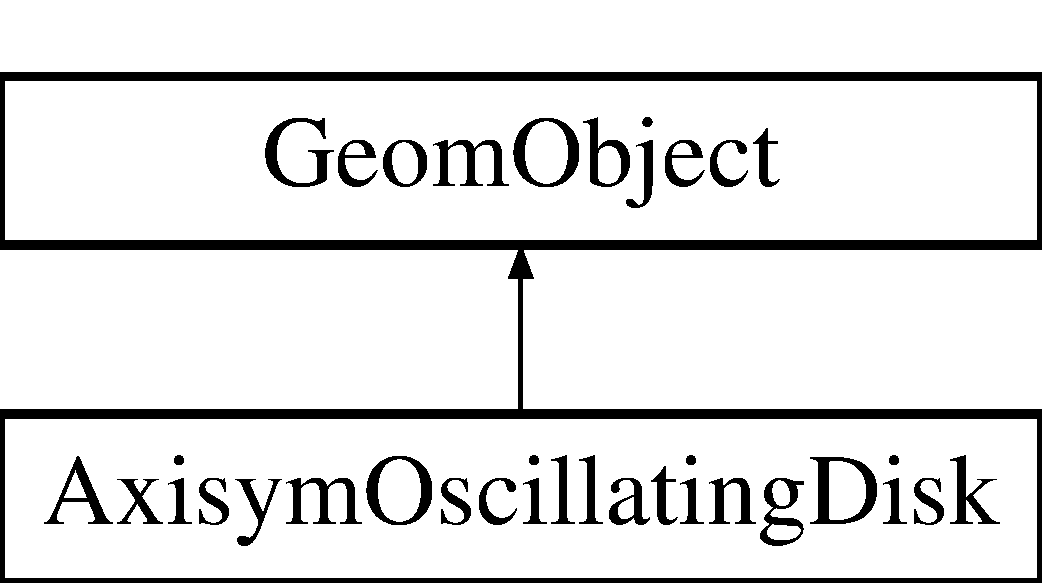
\includegraphics[height=2.000000cm]{classAxisymOscillatingDisk}
\end{center}
\end{figure}
\subsection*{Public Member Functions}
\begin{DoxyCompactItemize}
\item 
\hyperlink{classAxisymOscillatingDisk_a7671a9c1b8d4d854752ea14aa4f5865d}{Axisym\+Oscillating\+Disk} (const double \&ampl, const double \&nu, Time\+Stepper $\ast$time\+\_\+stepper\+\_\+pt)
\begin{DoxyCompactList}\small\item\em Constructor\+: 2 Lagrangian coordinate, 2 Eulerian coords. Pass amplitude of oscillation, Poisson ratio nu, and pointer to global timestepper. \end{DoxyCompactList}\item 
\hyperlink{classAxisymOscillatingDisk_ab79de13fa0dcfac5d04d6ff371241c5d}{$\sim$\+Axisym\+Oscillating\+Disk} ()
\begin{DoxyCompactList}\small\item\em Destructor (empty) \end{DoxyCompactList}\item 
void \hyperlink{classAxisymOscillatingDisk_ab63d762c8fecce8de5a2b7dc4b3b677a}{position} (const Vector$<$ double $>$ \&xi, Vector$<$ double $>$ \&r) const
\begin{DoxyCompactList}\small\item\em Position vector at Lagrangian coordinate xi at present time. \end{DoxyCompactList}\item 
void \hyperlink{classAxisymOscillatingDisk_a7b39985cb0658924472700f4383b53aa}{veloc} (const Vector$<$ double $>$ \&xi, Vector$<$ double $>$ \&veloc)
\begin{DoxyCompactList}\small\item\em Parametrised velocity on object at current time\+: veloc = d r(xi)/dt. \end{DoxyCompactList}\item 
void \hyperlink{classAxisymOscillatingDisk_a92993399b50f818c9045fe7cecf47fcb}{accel} (const Vector$<$ double $>$ \&xi, Vector$<$ double $>$ \&accel)
\begin{DoxyCompactList}\small\item\em Parametrised acceleration on object at current time\+: accel = d$^\wedge$2 r(xi)/dt$^\wedge$2. \end{DoxyCompactList}\item 
void \hyperlink{classAxisymOscillatingDisk_a47de8f45fc7006ccadb1300fefe54dfe}{dposition\+\_\+dt} (const Vector$<$ double $>$ \&xi, const unsigned \&j, Vector$<$ double $>$ \&drdt)
\begin{DoxyCompactList}\small\item\em Parametrised j-\/th time-\/derivative on object at current time\+: $ \frac{d^{j} r(\zeta)}{dt^j} $. \end{DoxyCompactList}\end{DoxyCompactItemize}
\subsection*{Static Public Member Functions}
\begin{DoxyCompactItemize}
\item 
static void \hyperlink{classAxisymOscillatingDisk_ae6a90b479781b587bb8905e7bf2bba3b}{residual\+\_\+for\+\_\+dispersion} (const Vector$<$ double $>$ \&param, const Vector$<$ double $>$ \&omega, Vector$<$ double $>$ \&residual)
\begin{DoxyCompactList}\small\item\em Residual of dispersion relation for use in black-\/box Newton method which requires global (or static) functions. Poisson\textquotesingle{}s ratio is passed as parameter. \end{DoxyCompactList}\end{DoxyCompactItemize}
\subsection*{Private Attributes}
\begin{DoxyCompactItemize}
\item 
double \hyperlink{classAxisymOscillatingDisk_a9b73de59d11877c96bc85ad52fe7c407}{Ampl}
\begin{DoxyCompactList}\small\item\em Amplitude of oscillation. \end{DoxyCompactList}\item 
double \hyperlink{classAxisymOscillatingDisk_a7789dcf51ef2e2eb6e5eaa826f404da1}{T}
\begin{DoxyCompactList}\small\item\em Period of oscillation. \end{DoxyCompactList}\item 
double \hyperlink{classAxisymOscillatingDisk_abe977725f5fc04c5bfa8466ecdef0956}{Nu}
\begin{DoxyCompactList}\small\item\em Poisson ratio nu. \end{DoxyCompactList}\item 
double \hyperlink{classAxisymOscillatingDisk_ab0ae3a1a7324dd0ccce15fd84471e3d1}{Omega}
\begin{DoxyCompactList}\small\item\em Eigenfrequency. \end{DoxyCompactList}\end{DoxyCompactItemize}


\subsection{Detailed Description}
Axisymmetrially oscillating disk with displacement field according to linear elasticity. 

Definition at line 88 of file disk\+\_\+oscillation.\+cc.



\subsection{Constructor \& Destructor Documentation}
\mbox{\Hypertarget{classAxisymOscillatingDisk_a7671a9c1b8d4d854752ea14aa4f5865d}\label{classAxisymOscillatingDisk_a7671a9c1b8d4d854752ea14aa4f5865d}} 
\index{Axisym\+Oscillating\+Disk@{Axisym\+Oscillating\+Disk}!Axisym\+Oscillating\+Disk@{Axisym\+Oscillating\+Disk}}
\index{Axisym\+Oscillating\+Disk@{Axisym\+Oscillating\+Disk}!Axisym\+Oscillating\+Disk@{Axisym\+Oscillating\+Disk}}
\subsubsection{\texorpdfstring{Axisym\+Oscillating\+Disk()}{AxisymOscillatingDisk()}}
{\footnotesize\ttfamily Axisym\+Oscillating\+Disk\+::\+Axisym\+Oscillating\+Disk (\begin{DoxyParamCaption}\item[{const double \&}]{ampl,  }\item[{const double \&}]{nu,  }\item[{Time\+Stepper $\ast$}]{time\+\_\+stepper\+\_\+pt }\end{DoxyParamCaption})}



Constructor\+: 2 Lagrangian coordinate, 2 Eulerian coords. Pass amplitude of oscillation, Poisson ratio nu, and pointer to global timestepper. 

Constructor\+: 2 Lagrangian coordinates, 2 Eulerian coords. Pass amplitude of oscillation, Poisson ratio nu, and pointer to global timestepper. 

Definition at line 177 of file disk\+\_\+oscillation.\+cc.



References Nu, Omega, residual\+\_\+for\+\_\+dispersion(), and T.



Referenced by Disk\+Oscillation\+Problem$<$ E\+L\+E\+M\+E\+N\+T $>$\+::run().

\mbox{\Hypertarget{classAxisymOscillatingDisk_ab79de13fa0dcfac5d04d6ff371241c5d}\label{classAxisymOscillatingDisk_ab79de13fa0dcfac5d04d6ff371241c5d}} 
\index{Axisym\+Oscillating\+Disk@{Axisym\+Oscillating\+Disk}!````~Axisym\+Oscillating\+Disk@{$\sim$\+Axisym\+Oscillating\+Disk}}
\index{````~Axisym\+Oscillating\+Disk@{$\sim$\+Axisym\+Oscillating\+Disk}!Axisym\+Oscillating\+Disk@{Axisym\+Oscillating\+Disk}}
\subsubsection{\texorpdfstring{$\sim$\+Axisym\+Oscillating\+Disk()}{~AxisymOscillatingDisk()}}
{\footnotesize\ttfamily Axisym\+Oscillating\+Disk\+::$\sim$\+Axisym\+Oscillating\+Disk (\begin{DoxyParamCaption}{ }\end{DoxyParamCaption})\hspace{0.3cm}{\ttfamily [inline]}}



Destructor (empty) 



Definition at line 100 of file disk\+\_\+oscillation.\+cc.



\subsection{Member Function Documentation}
\mbox{\Hypertarget{classAxisymOscillatingDisk_a92993399b50f818c9045fe7cecf47fcb}\label{classAxisymOscillatingDisk_a92993399b50f818c9045fe7cecf47fcb}} 
\index{Axisym\+Oscillating\+Disk@{Axisym\+Oscillating\+Disk}!accel@{accel}}
\index{accel@{accel}!Axisym\+Oscillating\+Disk@{Axisym\+Oscillating\+Disk}}
\subsubsection{\texorpdfstring{accel()}{accel()}}
{\footnotesize\ttfamily void Axisym\+Oscillating\+Disk\+::accel (\begin{DoxyParamCaption}\item[{const Vector$<$ double $>$ \&}]{xi,  }\item[{Vector$<$ double $>$ \&}]{accel }\end{DoxyParamCaption})}



Parametrised acceleration on object at current time\+: accel = d$^\wedge$2 r(xi)/dt$^\wedge$2. 

Parametrised acceleration on object at current time\+: accel = d$^\wedge$2 r(xi)/dt$^\wedge$2. 

Definition at line 287 of file disk\+\_\+oscillation.\+cc.



References Ampl, Omega, and T.

\mbox{\Hypertarget{classAxisymOscillatingDisk_a47de8f45fc7006ccadb1300fefe54dfe}\label{classAxisymOscillatingDisk_a47de8f45fc7006ccadb1300fefe54dfe}} 
\index{Axisym\+Oscillating\+Disk@{Axisym\+Oscillating\+Disk}!dposition\+\_\+dt@{dposition\+\_\+dt}}
\index{dposition\+\_\+dt@{dposition\+\_\+dt}!Axisym\+Oscillating\+Disk@{Axisym\+Oscillating\+Disk}}
\subsubsection{\texorpdfstring{dposition\+\_\+dt()}{dposition\_dt()}}
{\footnotesize\ttfamily void Axisym\+Oscillating\+Disk\+::dposition\+\_\+dt (\begin{DoxyParamCaption}\item[{const Vector$<$ double $>$ \&}]{xi,  }\item[{const unsigned \&}]{j,  }\item[{Vector$<$ double $>$ \&}]{drdt }\end{DoxyParamCaption})\hspace{0.3cm}{\ttfamily [inline]}}



Parametrised j-\/th time-\/derivative on object at current time\+: $ \frac{d^{j} r(\zeta)}{dt^j} $. 



Definition at line 115 of file disk\+\_\+oscillation.\+cc.

\mbox{\Hypertarget{classAxisymOscillatingDisk_ab63d762c8fecce8de5a2b7dc4b3b677a}\label{classAxisymOscillatingDisk_ab63d762c8fecce8de5a2b7dc4b3b677a}} 
\index{Axisym\+Oscillating\+Disk@{Axisym\+Oscillating\+Disk}!position@{position}}
\index{position@{position}!Axisym\+Oscillating\+Disk@{Axisym\+Oscillating\+Disk}}
\subsubsection{\texorpdfstring{position()}{position()}}
{\footnotesize\ttfamily void Axisym\+Oscillating\+Disk\+::position (\begin{DoxyParamCaption}\item[{const Vector$<$ double $>$ \&}]{xi,  }\item[{Vector$<$ double $>$ \&}]{r }\end{DoxyParamCaption}) const}



Position vector at Lagrangian coordinate xi at present time. 

Position Vector at Lagrangian coordinate xi at present time. 

Definition at line 210 of file disk\+\_\+oscillation.\+cc.



References Ampl, Omega, and T.

\mbox{\Hypertarget{classAxisymOscillatingDisk_ae6a90b479781b587bb8905e7bf2bba3b}\label{classAxisymOscillatingDisk_ae6a90b479781b587bb8905e7bf2bba3b}} 
\index{Axisym\+Oscillating\+Disk@{Axisym\+Oscillating\+Disk}!residual\+\_\+for\+\_\+dispersion@{residual\+\_\+for\+\_\+dispersion}}
\index{residual\+\_\+for\+\_\+dispersion@{residual\+\_\+for\+\_\+dispersion}!Axisym\+Oscillating\+Disk@{Axisym\+Oscillating\+Disk}}
\subsubsection{\texorpdfstring{residual\+\_\+for\+\_\+dispersion()}{residual\_for\_dispersion()}}
{\footnotesize\ttfamily void Axisym\+Oscillating\+Disk\+::residual\+\_\+for\+\_\+dispersion (\begin{DoxyParamCaption}\item[{const Vector$<$ double $>$ \&}]{param,  }\item[{const Vector$<$ double $>$ \&}]{omega,  }\item[{Vector$<$ double $>$ \&}]{residual }\end{DoxyParamCaption})\hspace{0.3cm}{\ttfamily [static]}}



Residual of dispersion relation for use in black-\/box Newton method which requires global (or static) functions. Poisson\textquotesingle{}s ratio is passed as parameter. 

Residual of dispersion relation for use in black box Newton method which requires global (or static) functions. Poisson\textquotesingle{}s ratio is passed as parameter. 

Definition at line 327 of file disk\+\_\+oscillation.\+cc.



Referenced by Axisym\+Oscillating\+Disk().

\mbox{\Hypertarget{classAxisymOscillatingDisk_a7b39985cb0658924472700f4383b53aa}\label{classAxisymOscillatingDisk_a7b39985cb0658924472700f4383b53aa}} 
\index{Axisym\+Oscillating\+Disk@{Axisym\+Oscillating\+Disk}!veloc@{veloc}}
\index{veloc@{veloc}!Axisym\+Oscillating\+Disk@{Axisym\+Oscillating\+Disk}}
\subsubsection{\texorpdfstring{veloc()}{veloc()}}
{\footnotesize\ttfamily void Axisym\+Oscillating\+Disk\+::veloc (\begin{DoxyParamCaption}\item[{const Vector$<$ double $>$ \&}]{xi,  }\item[{Vector$<$ double $>$ \&}]{veloc }\end{DoxyParamCaption})}



Parametrised velocity on object at current time\+: veloc = d r(xi)/dt. 



Definition at line 248 of file disk\+\_\+oscillation.\+cc.



References Ampl, Omega, and T.



\subsection{Member Data Documentation}
\mbox{\Hypertarget{classAxisymOscillatingDisk_a9b73de59d11877c96bc85ad52fe7c407}\label{classAxisymOscillatingDisk_a9b73de59d11877c96bc85ad52fe7c407}} 
\index{Axisym\+Oscillating\+Disk@{Axisym\+Oscillating\+Disk}!Ampl@{Ampl}}
\index{Ampl@{Ampl}!Axisym\+Oscillating\+Disk@{Axisym\+Oscillating\+Disk}}
\subsubsection{\texorpdfstring{Ampl}{Ampl}}
{\footnotesize\ttfamily double Axisym\+Oscillating\+Disk\+::\+Ampl\hspace{0.3cm}{\ttfamily [private]}}



Amplitude of oscillation. 



Definition at line 156 of file disk\+\_\+oscillation.\+cc.



Referenced by accel(), position(), and veloc().

\mbox{\Hypertarget{classAxisymOscillatingDisk_abe977725f5fc04c5bfa8466ecdef0956}\label{classAxisymOscillatingDisk_abe977725f5fc04c5bfa8466ecdef0956}} 
\index{Axisym\+Oscillating\+Disk@{Axisym\+Oscillating\+Disk}!Nu@{Nu}}
\index{Nu@{Nu}!Axisym\+Oscillating\+Disk@{Axisym\+Oscillating\+Disk}}
\subsubsection{\texorpdfstring{Nu}{Nu}}
{\footnotesize\ttfamily double Axisym\+Oscillating\+Disk\+::\+Nu\hspace{0.3cm}{\ttfamily [private]}}



Poisson ratio nu. 



Definition at line 162 of file disk\+\_\+oscillation.\+cc.



Referenced by Axisym\+Oscillating\+Disk().

\mbox{\Hypertarget{classAxisymOscillatingDisk_ab0ae3a1a7324dd0ccce15fd84471e3d1}\label{classAxisymOscillatingDisk_ab0ae3a1a7324dd0ccce15fd84471e3d1}} 
\index{Axisym\+Oscillating\+Disk@{Axisym\+Oscillating\+Disk}!Omega@{Omega}}
\index{Omega@{Omega}!Axisym\+Oscillating\+Disk@{Axisym\+Oscillating\+Disk}}
\subsubsection{\texorpdfstring{Omega}{Omega}}
{\footnotesize\ttfamily double Axisym\+Oscillating\+Disk\+::\+Omega\hspace{0.3cm}{\ttfamily [private]}}



Eigenfrequency. 



Definition at line 165 of file disk\+\_\+oscillation.\+cc.



Referenced by accel(), Axisym\+Oscillating\+Disk(), position(), and veloc().

\mbox{\Hypertarget{classAxisymOscillatingDisk_a7789dcf51ef2e2eb6e5eaa826f404da1}\label{classAxisymOscillatingDisk_a7789dcf51ef2e2eb6e5eaa826f404da1}} 
\index{Axisym\+Oscillating\+Disk@{Axisym\+Oscillating\+Disk}!T@{T}}
\index{T@{T}!Axisym\+Oscillating\+Disk@{Axisym\+Oscillating\+Disk}}
\subsubsection{\texorpdfstring{T}{T}}
{\footnotesize\ttfamily double Axisym\+Oscillating\+Disk\+::T\hspace{0.3cm}{\ttfamily [private]}}



Period of oscillation. 



Definition at line 159 of file disk\+\_\+oscillation.\+cc.



Referenced by accel(), Axisym\+Oscillating\+Disk(), position(), and veloc().



The documentation for this class was generated from the following file\+:\begin{DoxyCompactItemize}
\item 
\hyperlink{disk__oscillation_8cc}{disk\+\_\+oscillation.\+cc}\end{DoxyCompactItemize}

\hypertarget{classDiskOscillationProblem}{}\section{Disk\+Oscillation\+Problem$<$ E\+L\+E\+M\+E\+NT $>$ Class Template Reference}
\label{classDiskOscillationProblem}\index{Disk\+Oscillation\+Problem$<$ E\+L\+E\+M\+E\+N\+T $>$@{Disk\+Oscillation\+Problem$<$ E\+L\+E\+M\+E\+N\+T $>$}}


Problem class to simulate small-\/amplitude oscillations of a circular disk.  


Inheritance diagram for Disk\+Oscillation\+Problem$<$ E\+L\+E\+M\+E\+NT $>$\+:\begin{figure}[H]
\begin{center}
\leavevmode
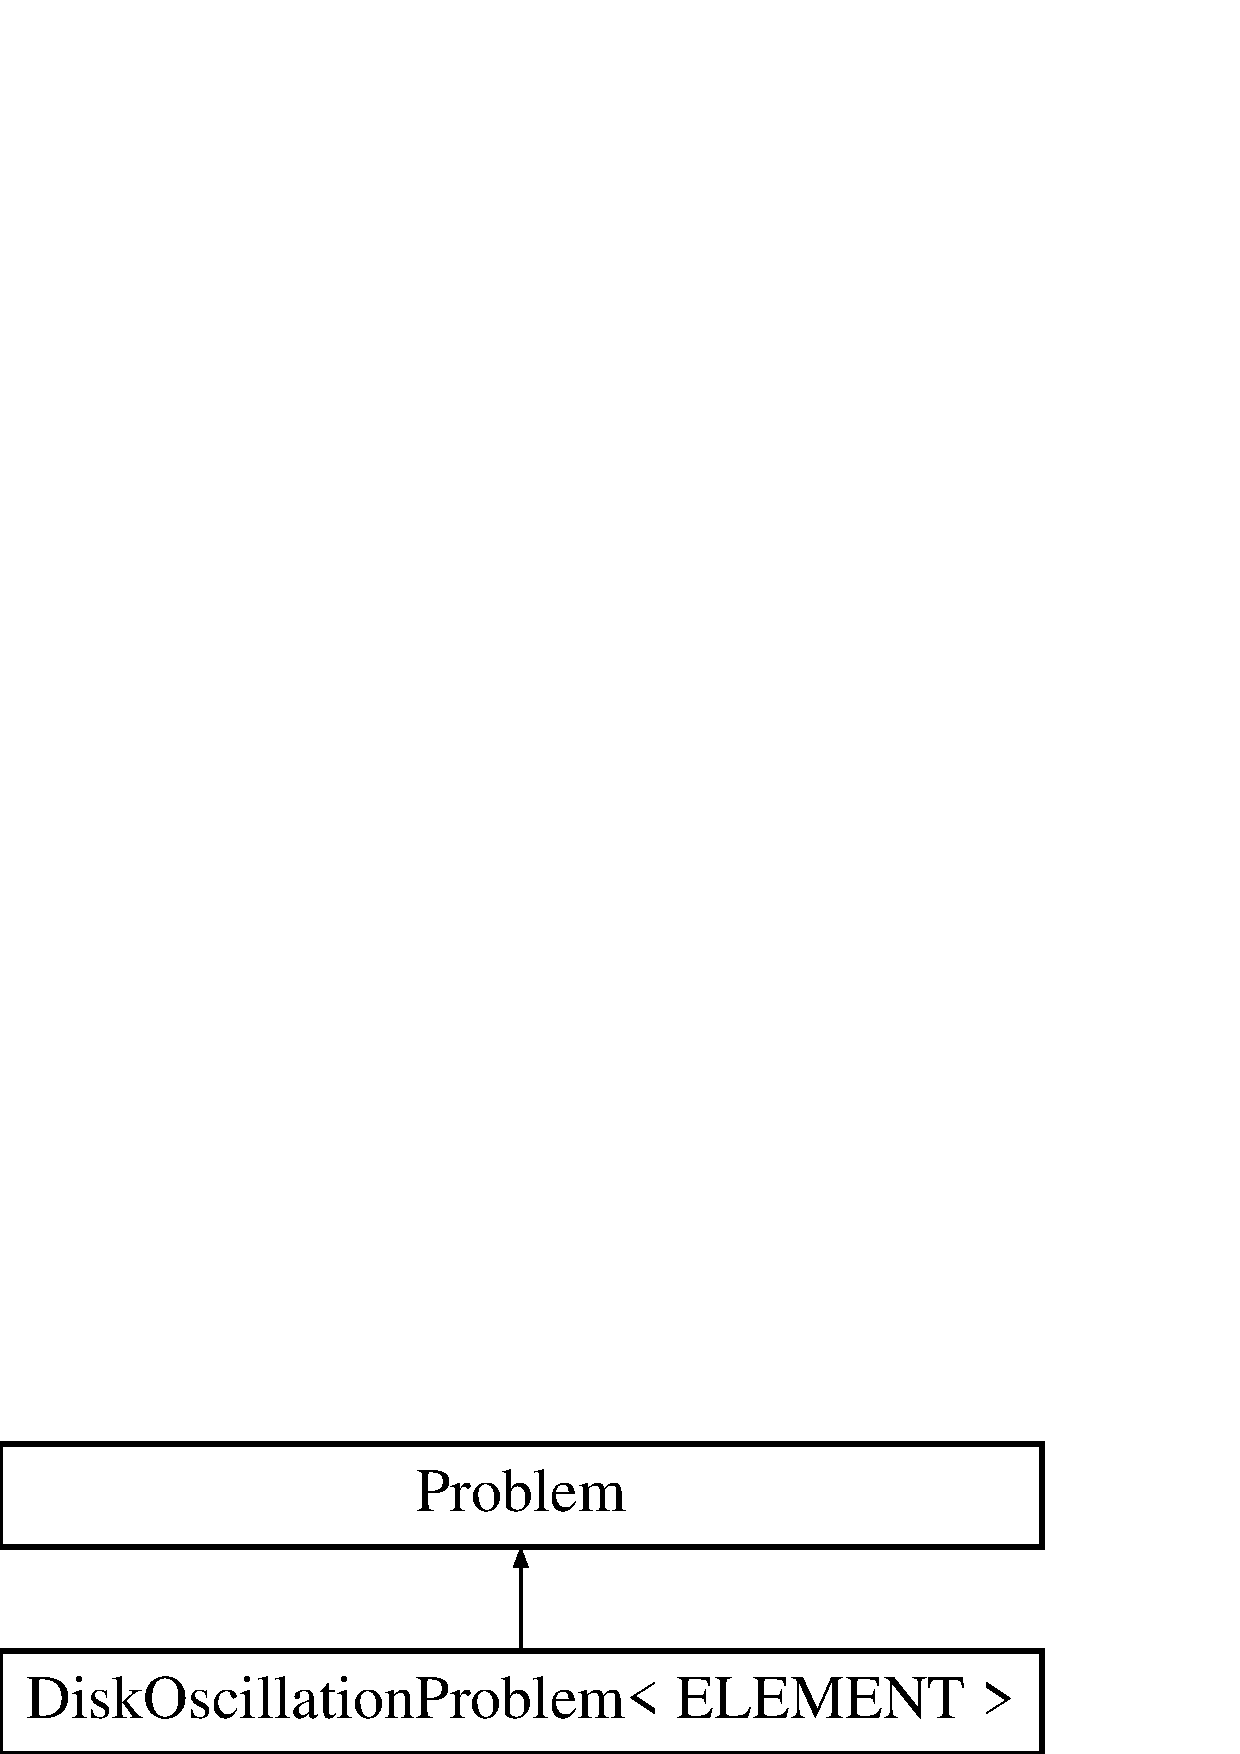
\includegraphics[height=2.000000cm]{classDiskOscillationProblem}
\end{center}
\end{figure}
\subsection*{Public Member Functions}
\begin{DoxyCompactItemize}
\item 
\hyperlink{classDiskOscillationProblem_a5ce89d95d655d8c5b579171c8e9a54b9}{Disk\+Oscillation\+Problem} ()
\begin{DoxyCompactList}\small\item\em Constructor. \end{DoxyCompactList}\item 
void \hyperlink{classDiskOscillationProblem_a84fdc4311e8cc1fa5f80dc5568c88413}{actions\+\_\+after\+\_\+newton\+\_\+solve} ()
\begin{DoxyCompactList}\small\item\em Update function (empty) \end{DoxyCompactList}\item 
void \hyperlink{classDiskOscillationProblem_afea297af1844657099dec3d717fcccc5}{actions\+\_\+before\+\_\+newton\+\_\+solve} ()
\begin{DoxyCompactList}\small\item\em Update function (empty) \end{DoxyCompactList}\item 
\hyperlink{classElasticRefineableQuarterCircleSectorMesh}{Elastic\+Refineable\+Quarter\+Circle\+Sector\+Mesh}$<$ E\+L\+E\+M\+E\+NT $>$ $\ast$ \hyperlink{classDiskOscillationProblem_a9de851f400e5c161c5abf8efb2f2b082}{mesh\+\_\+pt} ()
\begin{DoxyCompactList}\small\item\em Access function for the solid mesh. \end{DoxyCompactList}\item 
void \hyperlink{classDiskOscillationProblem_ac0f7b36ffffa73ee49bc95bd961835dd}{run} (const unsigned \&nstep)
\begin{DoxyCompactList}\small\item\em Run the problem\+: Pass number of timesteps to be performed. \end{DoxyCompactList}\item 
void \hyperlink{classDiskOscillationProblem_adf6e2bf1843d5f5e3fa7b2fc5fb129a8}{doc\+\_\+solution} (Doc\+Info \&doc\+\_\+info)
\begin{DoxyCompactList}\small\item\em Doc the solution. \end{DoxyCompactList}\end{DoxyCompactItemize}
\subsection*{Private Attributes}
\begin{DoxyCompactItemize}
\item 
ofstream \hyperlink{classDiskOscillationProblem_a45a4b574c10c6416b3b6be950713f505}{Trace\+\_\+file}
\begin{DoxyCompactList}\small\item\em Trace file. \end{DoxyCompactList}\item 
Vector$<$ Node $\ast$ $>$ \hyperlink{classDiskOscillationProblem_a141a79f41b33b19a6fca57793836e4da}{Trace\+\_\+node\+\_\+pt}
\begin{DoxyCompactList}\small\item\em Vector of pointers to nodes whose position we\textquotesingle{}re tracing. \end{DoxyCompactList}\item 
\hyperlink{classAxisymOscillatingDisk}{Axisym\+Oscillating\+Disk} $\ast$ \hyperlink{classDiskOscillationProblem_a338517a04848bb75252751df32879e40}{I\+C\+\_\+geom\+\_\+object\+\_\+pt}
\begin{DoxyCompactList}\small\item\em Geometric object that specifies the initial conditions. \end{DoxyCompactList}\end{DoxyCompactItemize}


\subsection{Detailed Description}
\subsubsection*{template$<$class E\+L\+E\+M\+E\+NT$>$\newline
class Disk\+Oscillation\+Problem$<$ E\+L\+E\+M\+E\+N\+T $>$}

Problem class to simulate small-\/amplitude oscillations of a circular disk. 

Definition at line 418 of file disk\+\_\+oscillation.\+cc.



\subsection{Constructor \& Destructor Documentation}
\mbox{\Hypertarget{classDiskOscillationProblem_a5ce89d95d655d8c5b579171c8e9a54b9}\label{classDiskOscillationProblem_a5ce89d95d655d8c5b579171c8e9a54b9}} 
\index{Disk\+Oscillation\+Problem@{Disk\+Oscillation\+Problem}!Disk\+Oscillation\+Problem@{Disk\+Oscillation\+Problem}}
\index{Disk\+Oscillation\+Problem@{Disk\+Oscillation\+Problem}!Disk\+Oscillation\+Problem@{Disk\+Oscillation\+Problem}}
\subsubsection{\texorpdfstring{Disk\+Oscillation\+Problem()}{DiskOscillationProblem()}}
{\footnotesize\ttfamily template$<$class E\+L\+E\+M\+E\+NT $>$ \\
\hyperlink{classDiskOscillationProblem}{Disk\+Oscillation\+Problem}$<$ E\+L\+E\+M\+E\+NT $>$\+::\hyperlink{classDiskOscillationProblem}{Disk\+Oscillation\+Problem} (\begin{DoxyParamCaption}{ }\end{DoxyParamCaption})}



Constructor. 



Definition at line 466 of file disk\+\_\+oscillation.\+cc.



References Global\+\_\+\+Physical\+\_\+\+Variables\+::\+Constitutive\+\_\+law\+\_\+pt, and Global\+\_\+\+Physical\+\_\+\+Variables\+::\+Lambda\+\_\+sq.



\subsection{Member Function Documentation}
\mbox{\Hypertarget{classDiskOscillationProblem_a84fdc4311e8cc1fa5f80dc5568c88413}\label{classDiskOscillationProblem_a84fdc4311e8cc1fa5f80dc5568c88413}} 
\index{Disk\+Oscillation\+Problem@{Disk\+Oscillation\+Problem}!actions\+\_\+after\+\_\+newton\+\_\+solve@{actions\+\_\+after\+\_\+newton\+\_\+solve}}
\index{actions\+\_\+after\+\_\+newton\+\_\+solve@{actions\+\_\+after\+\_\+newton\+\_\+solve}!Disk\+Oscillation\+Problem@{Disk\+Oscillation\+Problem}}
\subsubsection{\texorpdfstring{actions\+\_\+after\+\_\+newton\+\_\+solve()}{actions\_after\_newton\_solve()}}
{\footnotesize\ttfamily template$<$class E\+L\+E\+M\+E\+NT$>$ \\
void \hyperlink{classDiskOscillationProblem}{Disk\+Oscillation\+Problem}$<$ E\+L\+E\+M\+E\+NT $>$\+::actions\+\_\+after\+\_\+newton\+\_\+solve (\begin{DoxyParamCaption}{ }\end{DoxyParamCaption})\hspace{0.3cm}{\ttfamily [inline]}}



Update function (empty) 



Definition at line 427 of file disk\+\_\+oscillation.\+cc.

\mbox{\Hypertarget{classDiskOscillationProblem_afea297af1844657099dec3d717fcccc5}\label{classDiskOscillationProblem_afea297af1844657099dec3d717fcccc5}} 
\index{Disk\+Oscillation\+Problem@{Disk\+Oscillation\+Problem}!actions\+\_\+before\+\_\+newton\+\_\+solve@{actions\+\_\+before\+\_\+newton\+\_\+solve}}
\index{actions\+\_\+before\+\_\+newton\+\_\+solve@{actions\+\_\+before\+\_\+newton\+\_\+solve}!Disk\+Oscillation\+Problem@{Disk\+Oscillation\+Problem}}
\subsubsection{\texorpdfstring{actions\+\_\+before\+\_\+newton\+\_\+solve()}{actions\_before\_newton\_solve()}}
{\footnotesize\ttfamily template$<$class E\+L\+E\+M\+E\+NT$>$ \\
void \hyperlink{classDiskOscillationProblem}{Disk\+Oscillation\+Problem}$<$ E\+L\+E\+M\+E\+NT $>$\+::actions\+\_\+before\+\_\+newton\+\_\+solve (\begin{DoxyParamCaption}{ }\end{DoxyParamCaption})\hspace{0.3cm}{\ttfamily [inline]}}



Update function (empty) 



Definition at line 430 of file disk\+\_\+oscillation.\+cc.

\mbox{\Hypertarget{classDiskOscillationProblem_adf6e2bf1843d5f5e3fa7b2fc5fb129a8}\label{classDiskOscillationProblem_adf6e2bf1843d5f5e3fa7b2fc5fb129a8}} 
\index{Disk\+Oscillation\+Problem@{Disk\+Oscillation\+Problem}!doc\+\_\+solution@{doc\+\_\+solution}}
\index{doc\+\_\+solution@{doc\+\_\+solution}!Disk\+Oscillation\+Problem@{Disk\+Oscillation\+Problem}}
\subsubsection{\texorpdfstring{doc\+\_\+solution()}{doc\_solution()}}
{\footnotesize\ttfamily template$<$class E\+L\+E\+M\+E\+NT $>$ \\
void \hyperlink{classDiskOscillationProblem}{Disk\+Oscillation\+Problem}$<$ E\+L\+E\+M\+E\+NT $>$\+::doc\+\_\+solution (\begin{DoxyParamCaption}\item[{Doc\+Info \&}]{doc\+\_\+info }\end{DoxyParamCaption})}



Doc the solution. 



Definition at line 558 of file disk\+\_\+oscillation.\+cc.

\mbox{\Hypertarget{classDiskOscillationProblem_a9de851f400e5c161c5abf8efb2f2b082}\label{classDiskOscillationProblem_a9de851f400e5c161c5abf8efb2f2b082}} 
\index{Disk\+Oscillation\+Problem@{Disk\+Oscillation\+Problem}!mesh\+\_\+pt@{mesh\+\_\+pt}}
\index{mesh\+\_\+pt@{mesh\+\_\+pt}!Disk\+Oscillation\+Problem@{Disk\+Oscillation\+Problem}}
\subsubsection{\texorpdfstring{mesh\+\_\+pt()}{mesh\_pt()}}
{\footnotesize\ttfamily template$<$class E\+L\+E\+M\+E\+NT$>$ \\
\hyperlink{classElasticRefineableQuarterCircleSectorMesh}{Elastic\+Refineable\+Quarter\+Circle\+Sector\+Mesh}$<$E\+L\+E\+M\+E\+NT$>$$\ast$ \hyperlink{classDiskOscillationProblem}{Disk\+Oscillation\+Problem}$<$ E\+L\+E\+M\+E\+NT $>$\+::mesh\+\_\+pt (\begin{DoxyParamCaption}{ }\end{DoxyParamCaption})\hspace{0.3cm}{\ttfamily [inline]}}



Access function for the solid mesh. 



Definition at line 433 of file disk\+\_\+oscillation.\+cc.

\mbox{\Hypertarget{classDiskOscillationProblem_ac0f7b36ffffa73ee49bc95bd961835dd}\label{classDiskOscillationProblem_ac0f7b36ffffa73ee49bc95bd961835dd}} 
\index{Disk\+Oscillation\+Problem@{Disk\+Oscillation\+Problem}!run@{run}}
\index{run@{run}!Disk\+Oscillation\+Problem@{Disk\+Oscillation\+Problem}}
\subsubsection{\texorpdfstring{run()}{run()}}
{\footnotesize\ttfamily template$<$class E\+L\+E\+M\+E\+NT $>$ \\
void \hyperlink{classDiskOscillationProblem}{Disk\+Oscillation\+Problem}$<$ E\+L\+E\+M\+E\+NT $>$\+::run (\begin{DoxyParamCaption}\item[{const unsigned \&}]{nstep }\end{DoxyParamCaption})}



Run the problem\+: Pass number of timesteps to be performed. 



Definition at line 757 of file disk\+\_\+oscillation.\+cc.



References Axisym\+Oscillating\+Disk\+::\+Axisym\+Oscillating\+Disk(), Global\+\_\+\+Physical\+\_\+\+Variables\+::multiplier(), and Global\+\_\+\+Physical\+\_\+\+Variables\+::\+Nu.



Referenced by main().



\subsection{Member Data Documentation}
\mbox{\Hypertarget{classDiskOscillationProblem_a338517a04848bb75252751df32879e40}\label{classDiskOscillationProblem_a338517a04848bb75252751df32879e40}} 
\index{Disk\+Oscillation\+Problem@{Disk\+Oscillation\+Problem}!I\+C\+\_\+geom\+\_\+object\+\_\+pt@{I\+C\+\_\+geom\+\_\+object\+\_\+pt}}
\index{I\+C\+\_\+geom\+\_\+object\+\_\+pt@{I\+C\+\_\+geom\+\_\+object\+\_\+pt}!Disk\+Oscillation\+Problem@{Disk\+Oscillation\+Problem}}
\subsubsection{\texorpdfstring{I\+C\+\_\+geom\+\_\+object\+\_\+pt}{IC\_geom\_object\_pt}}
{\footnotesize\ttfamily template$<$class E\+L\+E\+M\+E\+NT$>$ \\
\hyperlink{classAxisymOscillatingDisk}{Axisym\+Oscillating\+Disk}$\ast$ \hyperlink{classDiskOscillationProblem}{Disk\+Oscillation\+Problem}$<$ E\+L\+E\+M\+E\+NT $>$\+::I\+C\+\_\+geom\+\_\+object\+\_\+pt\hspace{0.3cm}{\ttfamily [private]}}



Geometric object that specifies the initial conditions. 



Definition at line 454 of file disk\+\_\+oscillation.\+cc.

\mbox{\Hypertarget{classDiskOscillationProblem_a45a4b574c10c6416b3b6be950713f505}\label{classDiskOscillationProblem_a45a4b574c10c6416b3b6be950713f505}} 
\index{Disk\+Oscillation\+Problem@{Disk\+Oscillation\+Problem}!Trace\+\_\+file@{Trace\+\_\+file}}
\index{Trace\+\_\+file@{Trace\+\_\+file}!Disk\+Oscillation\+Problem@{Disk\+Oscillation\+Problem}}
\subsubsection{\texorpdfstring{Trace\+\_\+file}{Trace\_file}}
{\footnotesize\ttfamily template$<$class E\+L\+E\+M\+E\+NT$>$ \\
ofstream \hyperlink{classDiskOscillationProblem}{Disk\+Oscillation\+Problem}$<$ E\+L\+E\+M\+E\+NT $>$\+::Trace\+\_\+file\hspace{0.3cm}{\ttfamily [private]}}



Trace file. 



Definition at line 448 of file disk\+\_\+oscillation.\+cc.

\mbox{\Hypertarget{classDiskOscillationProblem_a141a79f41b33b19a6fca57793836e4da}\label{classDiskOscillationProblem_a141a79f41b33b19a6fca57793836e4da}} 
\index{Disk\+Oscillation\+Problem@{Disk\+Oscillation\+Problem}!Trace\+\_\+node\+\_\+pt@{Trace\+\_\+node\+\_\+pt}}
\index{Trace\+\_\+node\+\_\+pt@{Trace\+\_\+node\+\_\+pt}!Disk\+Oscillation\+Problem@{Disk\+Oscillation\+Problem}}
\subsubsection{\texorpdfstring{Trace\+\_\+node\+\_\+pt}{Trace\_node\_pt}}
{\footnotesize\ttfamily template$<$class E\+L\+E\+M\+E\+NT$>$ \\
Vector$<$Node$\ast$$>$ \hyperlink{classDiskOscillationProblem}{Disk\+Oscillation\+Problem}$<$ E\+L\+E\+M\+E\+NT $>$\+::Trace\+\_\+node\+\_\+pt\hspace{0.3cm}{\ttfamily [private]}}



Vector of pointers to nodes whose position we\textquotesingle{}re tracing. 



Definition at line 451 of file disk\+\_\+oscillation.\+cc.



The documentation for this class was generated from the following file\+:\begin{DoxyCompactItemize}
\item 
\hyperlink{disk__oscillation_8cc}{disk\+\_\+oscillation.\+cc}\end{DoxyCompactItemize}

\hypertarget{classElasticRefineableQuarterCircleSectorMesh}{}\section{Elastic\+Refineable\+Quarter\+Circle\+Sector\+Mesh$<$ E\+L\+E\+M\+E\+NT $>$ Class Template Reference}
\label{classElasticRefineableQuarterCircleSectorMesh}\index{Elastic\+Refineable\+Quarter\+Circle\+Sector\+Mesh$<$ E\+L\+E\+M\+E\+N\+T $>$@{Elastic\+Refineable\+Quarter\+Circle\+Sector\+Mesh$<$ E\+L\+E\+M\+E\+N\+T $>$}}
Inheritance diagram for Elastic\+Refineable\+Quarter\+Circle\+Sector\+Mesh$<$ E\+L\+E\+M\+E\+NT $>$\+:\begin{figure}[H]
\begin{center}
\leavevmode
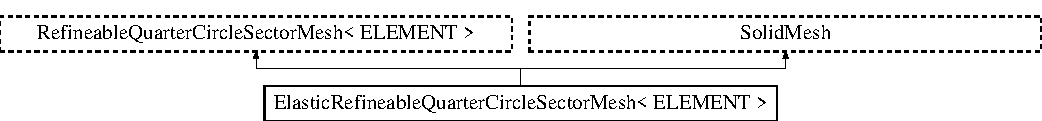
\includegraphics[height=1.623188cm]{classElasticRefineableQuarterCircleSectorMesh}
\end{center}
\end{figure}
\subsection*{Public Member Functions}
\begin{DoxyCompactItemize}
\item 
\hyperlink{classElasticRefineableQuarterCircleSectorMesh_a123699deecd2a908a7a882a9d2a9f4dd}{Elastic\+Refineable\+Quarter\+Circle\+Sector\+Mesh} (Geom\+Object $\ast$wall\+\_\+pt, const double \&xi\+\_\+lo, const double \&fract\+\_\+mid, const double \&xi\+\_\+hi, Time\+Stepper $\ast$time\+\_\+stepper\+\_\+pt=\&Mesh\+::\+Default\+\_\+\+Time\+Stepper)
\begin{DoxyCompactList}\small\item\em Constructor\+: Build mesh and copy Eulerian coords to Lagrangian ones so that the initial configuration is the stress-\/free one. \end{DoxyCompactList}\end{DoxyCompactItemize}


\subsection{Detailed Description}
\subsubsection*{template$<$class E\+L\+E\+M\+E\+NT$>$\newline
class Elastic\+Refineable\+Quarter\+Circle\+Sector\+Mesh$<$ E\+L\+E\+M\+E\+N\+T $>$}

Elastic quarter circle sector mesh\+: We \char`\"{}upgrade\char`\"{} the Refineable\+Quarter\+Circle\+Sector\+Mesh to become an Solid\+Mesh and equate the Eulerian and Lagrangian coordinates, thus making the domain represented by the mesh the stress-\/free configuration. 

Definition at line 363 of file disk\+\_\+oscillation.\+cc.



\subsection{Constructor \& Destructor Documentation}
\mbox{\Hypertarget{classElasticRefineableQuarterCircleSectorMesh_a123699deecd2a908a7a882a9d2a9f4dd}\label{classElasticRefineableQuarterCircleSectorMesh_a123699deecd2a908a7a882a9d2a9f4dd}} 
\index{Elastic\+Refineable\+Quarter\+Circle\+Sector\+Mesh@{Elastic\+Refineable\+Quarter\+Circle\+Sector\+Mesh}!Elastic\+Refineable\+Quarter\+Circle\+Sector\+Mesh@{Elastic\+Refineable\+Quarter\+Circle\+Sector\+Mesh}}
\index{Elastic\+Refineable\+Quarter\+Circle\+Sector\+Mesh@{Elastic\+Refineable\+Quarter\+Circle\+Sector\+Mesh}!Elastic\+Refineable\+Quarter\+Circle\+Sector\+Mesh@{Elastic\+Refineable\+Quarter\+Circle\+Sector\+Mesh}}
\subsubsection{\texorpdfstring{Elastic\+Refineable\+Quarter\+Circle\+Sector\+Mesh()}{ElasticRefineableQuarterCircleSectorMesh()}}
{\footnotesize\ttfamily template$<$class E\+L\+E\+M\+E\+NT$>$ \\
\hyperlink{classElasticRefineableQuarterCircleSectorMesh}{Elastic\+Refineable\+Quarter\+Circle\+Sector\+Mesh}$<$ E\+L\+E\+M\+E\+NT $>$\+::\hyperlink{classElasticRefineableQuarterCircleSectorMesh}{Elastic\+Refineable\+Quarter\+Circle\+Sector\+Mesh} (\begin{DoxyParamCaption}\item[{Geom\+Object $\ast$}]{wall\+\_\+pt,  }\item[{const double \&}]{xi\+\_\+lo,  }\item[{const double \&}]{fract\+\_\+mid,  }\item[{const double \&}]{xi\+\_\+hi,  }\item[{Time\+Stepper $\ast$}]{time\+\_\+stepper\+\_\+pt = {\ttfamily \&Mesh\+:\+:Default\+\_\+TimeStepper} }\end{DoxyParamCaption})\hspace{0.3cm}{\ttfamily [inline]}}



Constructor\+: Build mesh and copy Eulerian coords to Lagrangian ones so that the initial configuration is the stress-\/free one. 

Check that the element type is derived from the Solid\+Finite\+Element 

Definition at line 373 of file disk\+\_\+oscillation.\+cc.



The documentation for this class was generated from the following file\+:\begin{DoxyCompactItemize}
\item 
\hyperlink{disk__oscillation_8cc}{disk\+\_\+oscillation.\+cc}\end{DoxyCompactItemize}

\chapter{File Documentation}
\hypertarget{disk__oscillation_8cc}{}\section{disk\+\_\+oscillation.\+cc File Reference}
\label{disk__oscillation_8cc}\index{disk\+\_\+oscillation.\+cc@{disk\+\_\+oscillation.\+cc}}
\subsection*{Classes}
\begin{DoxyCompactItemize}
\item 
class \hyperlink{classAxisymOscillatingDisk}{Axisym\+Oscillating\+Disk}
\begin{DoxyCompactList}\small\item\em Axisymmetrially oscillating disk with displacement field according to linear elasticity. \end{DoxyCompactList}\item 
class \hyperlink{classElasticRefineableQuarterCircleSectorMesh}{Elastic\+Refineable\+Quarter\+Circle\+Sector\+Mesh$<$ E\+L\+E\+M\+E\+N\+T $>$}
\item 
class \hyperlink{classDiskOscillationProblem}{Disk\+Oscillation\+Problem$<$ E\+L\+E\+M\+E\+N\+T $>$}
\begin{DoxyCompactList}\small\item\em Problem class to simulate small-\/amplitude oscillations of a circular disk. \end{DoxyCompactList}\end{DoxyCompactItemize}
\subsection*{Namespaces}
\begin{DoxyCompactItemize}
\item 
 \hyperlink{namespaceGlobal__Physical__Variables}{Global\+\_\+\+Physical\+\_\+\+Variables}
\begin{DoxyCompactList}\small\item\em Global variables. \end{DoxyCompactList}\end{DoxyCompactItemize}
\subsection*{Functions}
\begin{DoxyCompactItemize}
\item 
double \hyperlink{namespaceGlobal__Physical__Variables_a01099bce3441c7fe79ac6926800097a8}{Global\+\_\+\+Physical\+\_\+\+Variables\+::multiplier} (const Vector$<$ double $>$ \&xi)
\begin{DoxyCompactList}\small\item\em Multiplier for inertia terms (needed for consistent assignment of initial conditions in Newmark scheme) \end{DoxyCompactList}\item 
int \hyperlink{disk__oscillation_8cc_a0ddf1224851353fc92bfbff6f499fa97}{main} (int argc, char $\ast$argv\mbox{[}$\,$\mbox{]})
\begin{DoxyCompactList}\small\item\em Driver for disk oscillation problem. \end{DoxyCompactList}\end{DoxyCompactItemize}
\subsection*{Variables}
\begin{DoxyCompactItemize}
\item 
double \hyperlink{namespaceGlobal__Physical__Variables_a3962c36313826b19f216f6bbbdd6a477}{Global\+\_\+\+Physical\+\_\+\+Variables\+::\+Nu} =0.\+3
\begin{DoxyCompactList}\small\item\em Poisson\textquotesingle{}s ratio. \end{DoxyCompactList}\item 
double \hyperlink{namespaceGlobal__Physical__Variables_a6fe17557ceb32dd353827fba60408363}{Global\+\_\+\+Physical\+\_\+\+Variables\+::\+Lambda\+\_\+sq} =(1.\+0-\/Nu)/((1.\+0+Nu)$\ast$(1.\+0-\/2.\+0$\ast$Nu))
\begin{DoxyCompactList}\small\item\em Timescale ratio. \end{DoxyCompactList}\item 
Constitutive\+Law $\ast$ \hyperlink{namespaceGlobal__Physical__Variables_a2a37fb040c832ee7a086bb13bb02a100}{Global\+\_\+\+Physical\+\_\+\+Variables\+::\+Constitutive\+\_\+law\+\_\+pt} =0
\begin{DoxyCompactList}\small\item\em Pointer to constitutive law. \end{DoxyCompactList}\end{DoxyCompactItemize}


\subsection{Function Documentation}
\mbox{\Hypertarget{disk__oscillation_8cc_a0ddf1224851353fc92bfbff6f499fa97}\label{disk__oscillation_8cc_a0ddf1224851353fc92bfbff6f499fa97}} 
\index{disk\+\_\+oscillation.\+cc@{disk\+\_\+oscillation.\+cc}!main@{main}}
\index{main@{main}!disk\+\_\+oscillation.\+cc@{disk\+\_\+oscillation.\+cc}}
\subsubsection{\texorpdfstring{main()}{main()}}
{\footnotesize\ttfamily int main (\begin{DoxyParamCaption}\item[{int}]{argc,  }\item[{char $\ast$}]{argv\mbox{[}$\,$\mbox{]} }\end{DoxyParamCaption})}



Driver for disk oscillation problem. 



Definition at line 819 of file disk\+\_\+oscillation.\+cc.



References Global\+\_\+\+Physical\+\_\+\+Variables\+::\+Constitutive\+\_\+law\+\_\+pt, Global\+\_\+\+Physical\+\_\+\+Variables\+::\+Nu, and Disk\+Oscillation\+Problem$<$ E\+L\+E\+M\+E\+N\+T $>$\+::run().


\hypertarget{disk__oscillation_8txt__doxygenified_8h}{}\section{disk\+\_\+oscillation.\+txt\+\_\+doxygenified.\+h File Reference}
\label{disk__oscillation_8txt__doxygenified_8h}\index{disk\+\_\+oscillation.\+txt\+\_\+doxygenified.\+h@{disk\+\_\+oscillation.\+txt\+\_\+doxygenified.\+h}}

%--- End generated contents ---

% Index
\backmatter
\newpage
\phantomsection
\clearemptydoublepage
\addcontentsline{toc}{chapter}{Index}
\printindex

\end{document}
